\documentclass{article}
\usepackage{graphicx}
\usepackage{pdfpages}
\usepackage{url}
\usepackage{savetrees}
\begin{document}
% Research into:
% - Eigenfaces
% - Sparse Low Rank Bilinear Discriminative Model
% - What are liveness tests
% - How can we test a system that we create?
% - What test data is available? ROSE-Youtu Face liveness detection dataset
% - Deep Learning based face liveness detection in videos
% - Cameras used: mobile cameras (most methods use average resolution images from webcams or camera phone)
% - "Deep learning based face liveness detection in videos" https://ieeexplore.ieee.org/document/8090202/
% - Ideas: texture based - an image of a face will have the facial textures, while the texture of a piece of paper is very different.
% - Video vs Photo. Wtih a video, you don't just use the subject image, but also factor in movement and changes.
    
    \paragraph{Title}
        Facial Liveness Testing for the Web - an analysis of different methods
    \paragraph{Project Type}
        Computer Vision, Image Processing and Security
    \paragraph{Description}
    In order to avoid spoofing in facial recognition systems, liveness tests are needed. While various liveness tests exist,
    some require specialized hardware and are therefore not suitable. This project aims to select the most suitable methods for
    a web facial authentication system, and analyze their effectiveness in terms of security. A liveness test is suitable if it
    uses only one built-in camera (found within laptops in the webcam, or in mobile devices as the front camera), and potentially
    the device screen (which varies in size depending on the device used), and can be done in near real time.
    \paragraph{Preliminary Preparation}
        \begin{itemize}
            \item Existing liveness tests
            \item What are the datasets available for testing/training of these liveness methods?
        \end{itemize}
    \paragraph{Minimum Objectives}
        \begin{itemize}
            \item Build the test framework, to test using several different datasets and liveness tests.
            \item Implement the image quality based liveness test.
            \item Train the classifier used within the image quality based liveness test.
            \item Evaluate the image quality liveness test.
        \end{itemize}
    \paragraph{Intermediate Objectives}
        \begin{itemize}
            \item Implement the eye tracking liveness test.
            \item Train the eye tracking liveness test classifier.
            \item Evaluate the eye tracking liveness test.
            \item Implement the CNN based liveness method (involving texture and temporal metrics).
            \item Train the CNN based liveness method classifier.
            \item Evaluate the CNN based liveness method.
            \item Compare all implemented methods together.
        \end{itemize}
    \paragraph{Advanced Objectives}
        \begin{itemize}
            \item Implement a consolodation layer, combining the metrics above through a classifier.
            \item Train the consolodation layer classifier
            \item Evaluate the performance of the consolodation layer compared to each method individually
            \item Implement the facial flashing liveness test.
        \end{itemize}
    \paragraph{References}
        \begin{itemize}
            \item Keras (\url{https://keras.io}) for Machine Learning
            \item OpenCV (\url{https://opencv.org/}) for Image Processing
            \item Image quality based liveness test (\url{https://ieeexplore.ieee.org/document/6671991})
            \item Eye tracking liveness test (\url{https://waset.org/publications/5308/liveness-detection-for-embedded-face-recognition-system})
            \item CNN based liveness test (\url{https://arxiv.org/pdf/1408.5601.pdf})
            \item Facial Flashing liveness test (\url{https://arxiv.org/pdf/1801.01949.pdf})
        \end{itemize}
   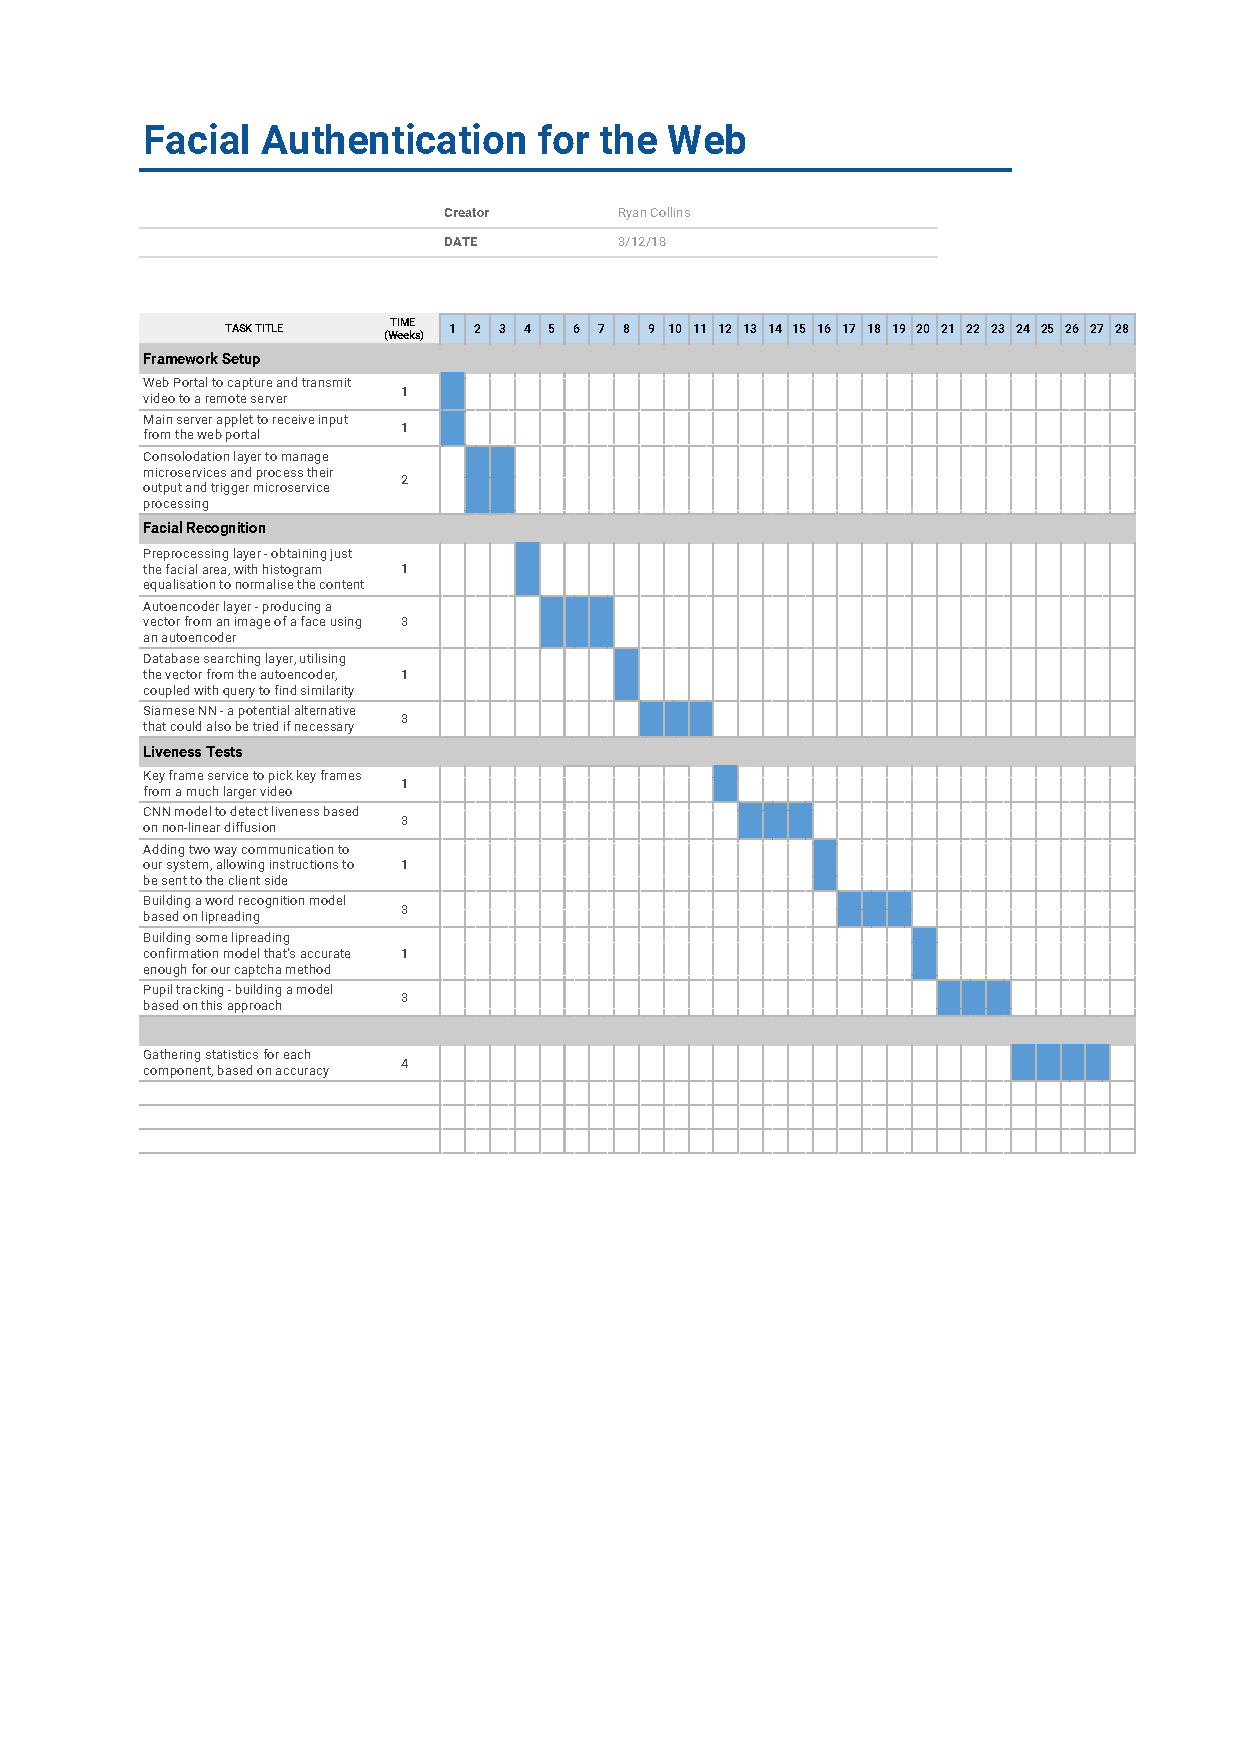
\includepdf{gantt.pdf}
\end{document}